\documentclass[10pt,twocolumn,letterpaper]{article}

\usepackage{cvpr}
\usepackage{times}
\usepackage{epsfig}
\usepackage{graphicx}
\graphicspath{{/home/li/图片/}}
\usepackage{amsmath}
\usepackage{amssymb}


\usepackage[breaklinks=true,bookmarks=false]{hyperref}

\cvprfinalcopy 

\def\cvprPaperID{****} 
\def\httilde{\mbox{\tt\raisebox{-.5ex}{\symbol{126}}}}

\setcounter{page}{4321}
\author{Qingyun Li\\
Changan University\\
May 27, 2018}        
\date{May 25, 2018}
\title{Image With Fog}
\begin{document}

\maketitle

\section{Formation of fog}
 \par As we all know, fog is a natural weather phenomenon. Especially recent yeays, due to the distruction of the   environment, this phenomenon is more and more serious. The buildings is higher and the air isn't free, all this reasons lead to the formation of the fog. And our common life has been effected seriously. 
 \par Fog consists of visible cloud water droplets or ice crystals suspended in the air at or near the Earth's surface\cite{gultepe2008fog}. So fog can be considered a type of low-lying cloud and is heavily influenced by nearby bodies of water, topography, and wind conditions.
 \par we can learn Concentration level of fog explicitly at the table 1.
\begin{table}[htbp]
\centering
\caption{Concentration level of fog}
\begin{tabular}{c|c}
\hline
Level & Horizontal Visibility Distence \\
\hline
mist & 1000-10000 \\
fog & 500-1000 \\
heavy fog & 200-500 \\
smoke fog & 50-200 \\
strong fog & <50 \\
\hline 
\end{tabular} 
\end{table}
\section{Smog}
 \par Given that the air pollution has been unprecedentedly severe in recent years, "smog" is more and more widly mentioned by everyone. This word is consist of two words, smoke and fog. We can learn it clearly from these words. Smog is different from fog, we can seen it at Fig.~\ref{difference}, and it's a type of air pollution derived from vehicular emission from internal combustion engines and industrial fumes that react inthe atmosphere with sunlight to form secondary pollutants that also combine with the primary emissions to form photochemical smog.
\begin{figure}[t]
\begin{center}
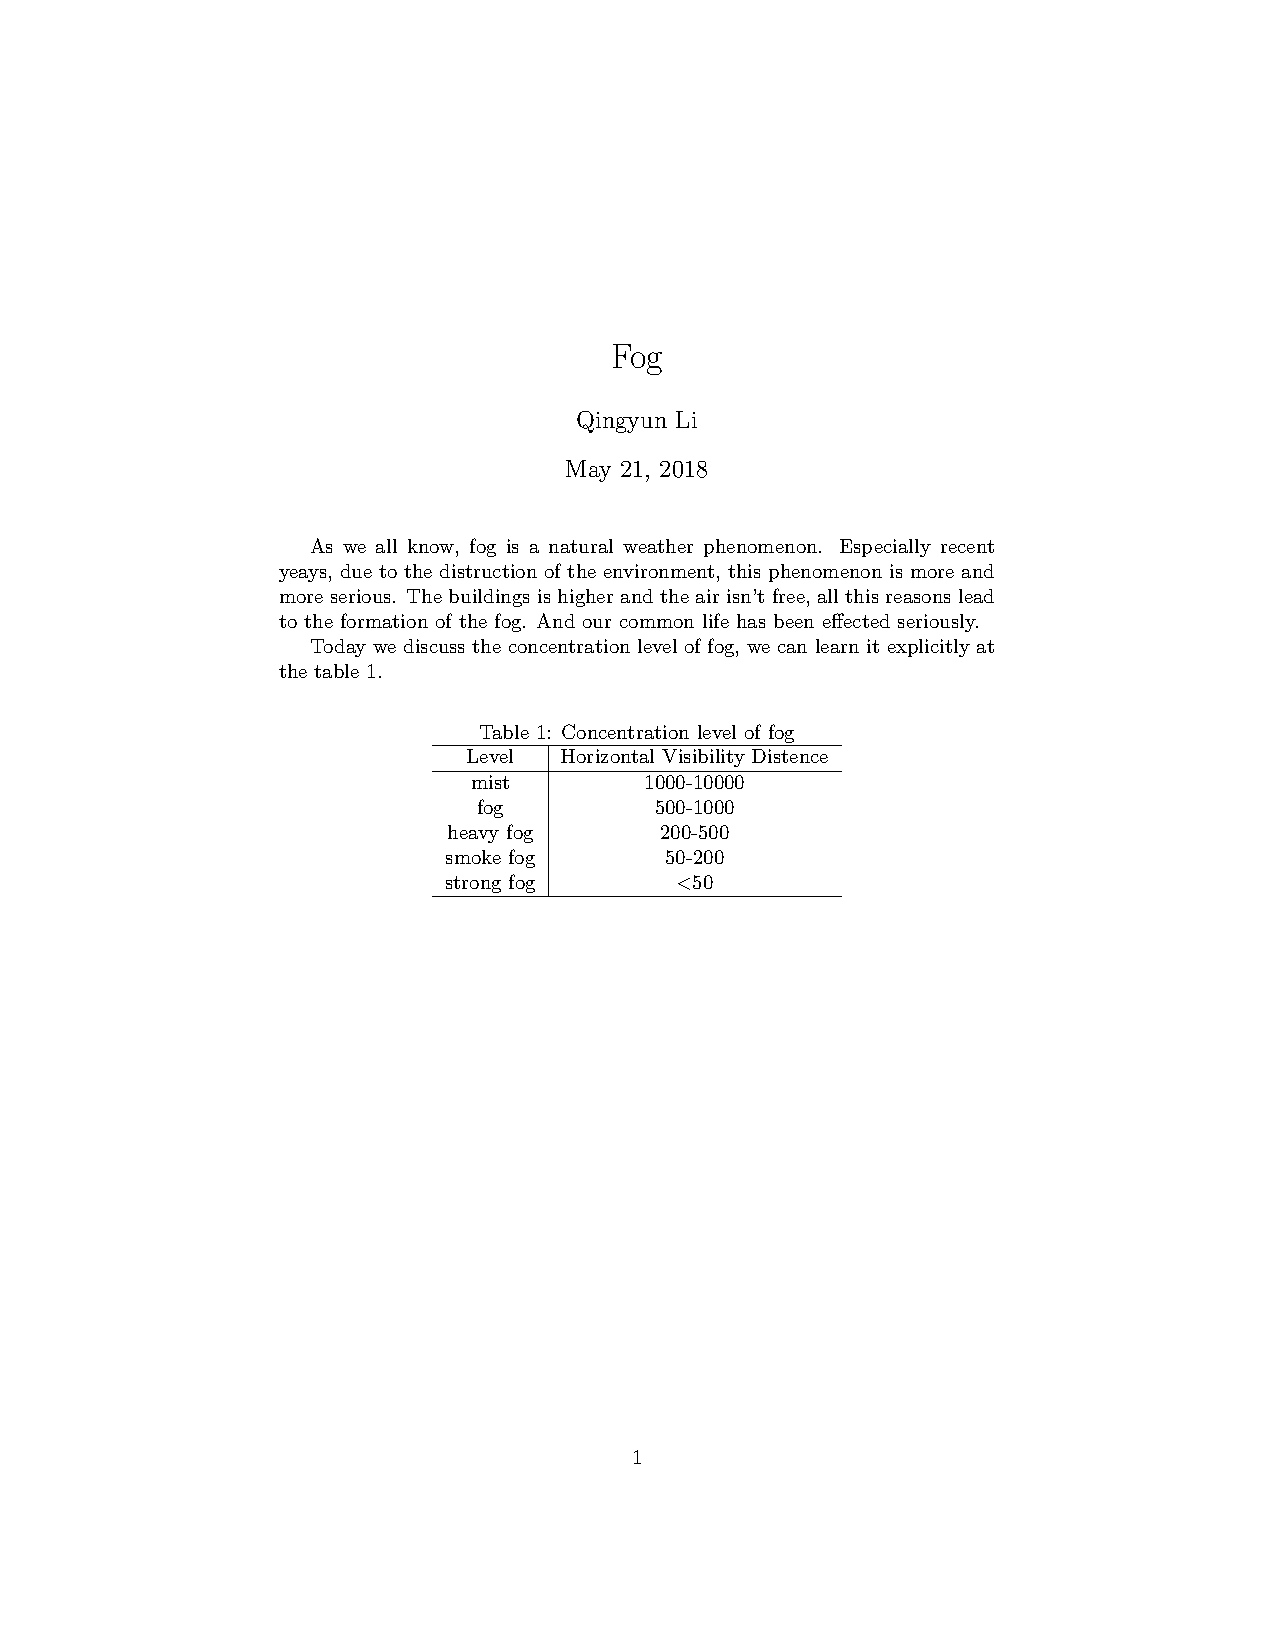
\includegraphics[width=0.4\textwidth]{Fog.jpeg} %\includegraphics[width=0.8\linewidth]{egfigure.eps}
\end{center}
   \caption{The difference of the fog and smog}
\label{difference}
\end{figure}
\section{Atmospheric light scattering model}
 \par The atmosphric light and the light reflected by the object itself combine with each other.And then, they enter the image acquisition device to form image.As is shown at Fig.~\ref{model1} So the suspended particles in the air and the incident light all effect the scattering effect of the atmosphere. When fog weather occurs, the amount of suspended particles increases. Therefore, in the process of image collection, the scattering and absorption of the radiated light is strengthened, and this resulted the color degradation and blurred details in the image.
\begin{figure}[htbp]
 \centering{}
\includegraphics[width=0.7\linewidth]{model1.jpeg}\\
 \caption{Atmospheric optical imaging model}
\label{model1}
\end{figure}
\section{Image degradation model}
 \par The degradation model is derived from the “Atmospheric light scattering model”, proposed by McCartney \emph{et al.}~\cite{Mccartney1976Optics}. A haze image formed as show in Fig.~\ref{model1} can be mathematically modeled as follows
\begin{equation}
I(x)=J(x)t(x)+A(1-t(x)) \label{eq1}
\end{equation}
\par This degradation model is consist of two parts, the first term of Eq.~\ref{eq1}, $J(x)t(x)$is the direct attenuation, and the second term of Eq.~\ref{eq1}, $A(1-t(x))$is the airlight.
\par The attenuation model means that the light reflection from the surface of the object encounters the sudpended particles and scatters, and part of the light deviates from the original direction, therefore, the incident light attenuates. This degree of attenuation is changes following the distance between the receiving device and the object. As the distance increases, the attenuation decays exponentially. The physical model is shown as Fig.~\ref{model2}.
\begin{figure}[htbp]
 \centering{}
\includegraphics[width=0.7\linewidth]{model2.jpg}\\
 \caption{The attenuation model}
\label{model2}
\end{figure}
\par The reflected light of the scene spots will attenuates because of the suspended particles, and at the same time, the sunlight and the reflected light of the ground will also scatter with the particles. This lead to the some of these light enters the receiving device and participates in imaging. These light called airlight. The physical model is shown as Fig.~\ref{model3}.  
\begin{figure}[htbp]
 \centering{}
\includegraphics[width=0.7\linewidth]{model3.jpg}\\
 \caption{Airlight}
\label{model3}
\end{figure} 
 \bibliographystyle{plain}
 \bibliography{single}
\end{document}
